The \emph{Message Passing Interface Standard} (\emph{MPI}) is a message passing library standard.
We might use it for machine parallelization if the tests show it gives better results than \emph{CAF} (see part \ref{sec:caf}).
In order to make the different machines communicate, it opens ssh connexions between them.
The general structure of a MPI program can be seen in figure \ref{fig:mpi_struct}.

\begin{figure}[H]
\centering
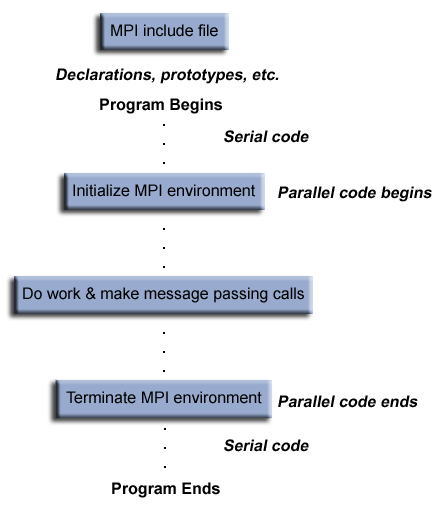
\includegraphics[width=.5\textwidth]{Parallelisation/Cluster/Img/prog_structure.png}
\caption{General MPI Program Structure. \cite{mpi_tuto}}
\label{fig:mpi_struct}
\end{figure}

MPI uses objects called communicators and groups to define which collection of processes may communicate with each other.
Within a communicator, every process has its own unique, integer identifier assigned by the system when the process initializes.
These ranks are used by the programmer to specify the source and destination of messages.

MPI allows for synchronized, blocking and non blocking routines.
Synchronized sending request only return after the message has been received, while blocking ones return after it is safe to modify the data in the sending buffer, and non blocking ones return immediately after sending the order, but offer no guarantee that it has already been executed.

Another type of routines handled by MPI is Collective Communication Routines.
They allow to make a similar operation on every process of a given communicator.
For example, it is possible to spread data from a single process to each other process, or on the contrary to regroup data from every process into a single one (as represented in figure \ref{fig:mpi_ccr}.
This will be especially useful for the algorithm, as it will require to regroup the results of every process (see part \ref{sec:paralstrat}).

\begin{figure}[H]
\centering
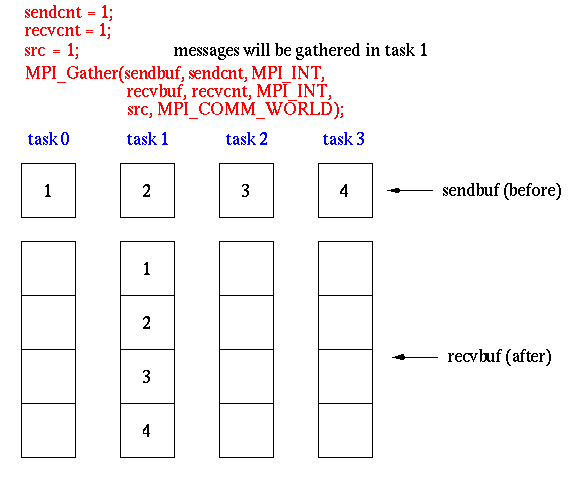
\includegraphics[width=.6\textwidth]{Parallelisation/Cluster/Img/MPI_Gather.png}
\caption{Example of a Collective Communication Routine. \cite{mpi_tuto}}
\label{fig:mpi_ccr}
\end{figure}